\section{System Model}
%----------------------------------------------------------------------------------------%
\subsection{Network Model}
We have Access Points (AP) and Edge Servers (ES) denoted as $\apSet \define \set{1,\dots,K}$ and $\mathcal{M} \define \set{1,\dots,M}$ respectively in our MEC (mobile edge computing) system depicted in Fig. \ref{fig:system}. In this system, we adopt the same timing mechanism at both AP and ES side with a minimum \emph{timeslot} lasting for $\tau$ seconds.

\begin{figure}[ht]
    \centering
    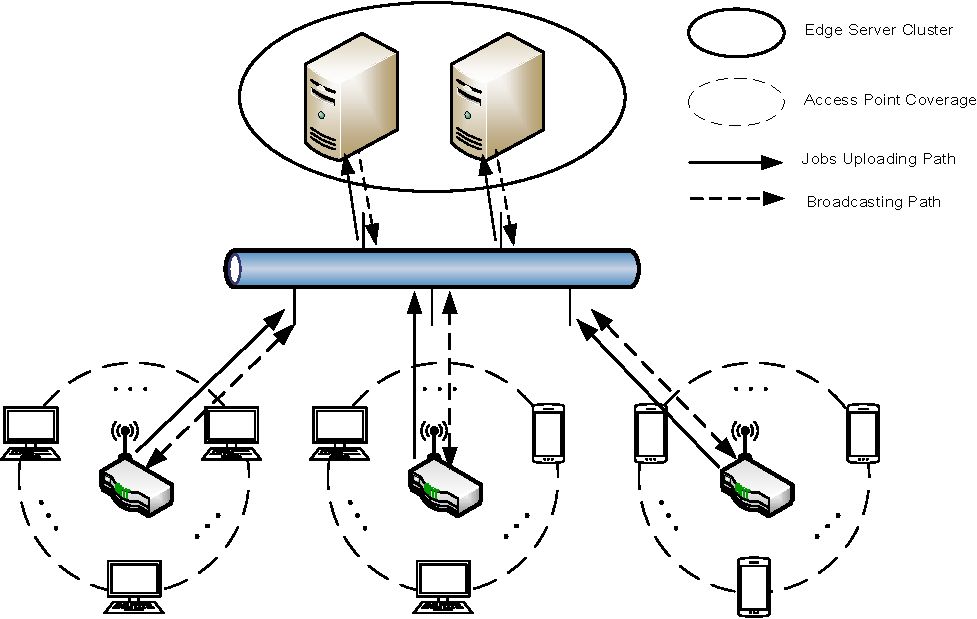
\includegraphics[width=0.45\textwidth]{system-model.pdf}
    \caption{The Illustration of MEC System Model}
    \label{fig:system}
\end{figure}

The User Equipment (UE) would offload the computation jobs on demand to the AP it connect.
We consider some types of jobs are supported on edge servers with Virtual Machine (VM) resources. The job space is denoted as $\jSpace \define \set{1,\dots, J}$, and jobs type distribution on each AP node follows the same distribution over $\jSpace$.
% which is obtained by statistics and denoted as $p_j \define \Pr\{\text{"j-type arrival"}\}$, where $\sum_{j\in\jSpace} p_j=1$.
Thus the job arrival process on $k$-th AP ($\forall k\in\apSet$) is compounded of the job arrivals from all UE connected, which follows the assumption as:
\begin{assumption}[Job Arrival Process for AP]
    The $j$-type job arrival distribution for $k$-th AP is denoted as $A_{k,j}$, which is independent and identically distributed (i.i.d) over each timeslot as $A_{k,j}$ following Poisson Point Process with intensity $\lambda_{k,j}$ ($\lambda_{k,j} > 0$). Thus average arrival rate of $j$-type jobs on $k$-th AP is $\mathbb{E}[A_{k,j}]=\lambda_{k,j}$, which implies that the occurrence average number of jobs in one timeslot would be $\lambda_{k,j}\tau$, .
\end{assumption}

The AP itself is assumed with no computation capability, and thus it need to further dispatch those jobs to the edge servers.
The jobs arrival in each timeslot on AP will be immediately dispatched to edge servers.
The corresponding uploading delay of one job is \emph{deterministic and job-type dependent} over one AP-ES link, which is denoted as $u_{k,m}(j)$ from $k$-th AP to $m$-th ES ($\forall k\in\apSet, \forall m\in\esSet$).

After arrival on edge servers, the jobs will join computation queue with the supported VM.
Each VM is considered running parallel without resource contention, and the jobs scheduling for each VM is with a single queue following \emph{FCFS} (First-Come-First-Serve).
{\color{red}The maximum queue length is set to discourage too many jobs pending on edge servers and is denoted as $L_Q$. The job submission over the limit will be rejected and announce the AP where the job is from.}

{\color{red}For jobs processing on edge servers, we adopt \emph{unrelated machines} assumption in \cite{tan-online}, where the job processing time on different servers are machine dependent and variant of resource or VM (virtual machine) constraints.
Moreover, we have $l_{m,j}$ to denote the processing time for $j$-type job on $m$-th edge serer following some distribution, whose largest processing time is bounded by $l_C$.}
For convenience, we assign type of jobs on edge servers which have no VM resource available with \emph{infinity} processing time, and this kind of dispatching possibility will be rejected at the AP side.
%----------------------------------------------------------------------------------------%

\subsection{Information-Sharing Broadcast Model}
As there is no centralized agent to distribute dispatching decisions to each AP node, an efficient information sharing scheme is needed to help collect global information and establish cooperation among standalone nodes.
In this paper, the proposed sharing scheme is designed via periodic broadcasting, where all the AP and ES nodes in the system should broadcast their system related information with a same period interval as $t_B$. More specifically, the broadcasting is applied in a synchronized way that all the nodes start to broadcast at the start of same timeslot and repeat broadcasting after the same periodic interval $t_B$. We call each periodic point of broadcasting as \emph{broadcast point} and denote the $i$-th broadcast with $t_i$ where,
\begin{align}
    t_i = i \cdot t_B, i=0,1,2,\dots
\end{align}
For $i$-th \emph{broadcast point}, the composed broadcast information from all the AP and ES nodes, and the corresponding information is listed as follows.
\begin{itemize}
    \item The $k$-th AP ($\forall k\in\apSet$) contains information $\mat{R}_k(i) \define (r^{(k)}_{m,j}(i))_{\set{m\in\esSet,j\in\jSpace}}$, where $r^{(k)}_{m,j}(i)$ denotes the remaining number of $j$-type jobs in uploading to $m$-th ES at time $t_i$; and we have $\vec{r}^{(k)}_{m} \define (r^{(k)}_{m,j}(i))_{j\in\jSpace}$ to denote the rows in $\vec{R}_k(i)$;
    \item The $m$-th ES ($\forall m\in\esSet$) contains information $\vec{Q}_m(i) \define \set{Q_{m,j}(i)|\forall j\in\jSpace}$ to denote the computation queues for different job types, where $Q_{m,j}(i) \define (q_{m,j}(i), \delta_{m,j}(i))$ to characterize the $j$-type FIFO queue on $m$-th ES; $q_{m,j}(i)$ denotes the number of $j$-type job queueing on $m$-th ES, and $\delta_{m,j}(i)$ denotes the remaining processing time for last job.
\end{itemize}
Thus the composed broadcasting information is denoted as:
\begin{align}
    \Obsv_i \define
        \Brace{
            \set{\mat{R}_{k}(i)|\forall k\in\apSet},
            \set{\vec{Q}_m(i)|\forall m\in\esSet}
        },
\end{align}
where $\Obsv_i$ is a set of global information of $i$-th broadcast. And it's actually the global system states at $t_i$.

We consider different AP nodes would receive partial broadcast information at different time points in one broadcast interval.
Let $d^{(p)}_{k,k'}$ denotes the broadcast delay between two AP nodes from $k'$-th AP to $k$-th AP ($\forall k,k'\in\apSet$); let $d^{(s)}_{k,m}$ denotes the broadcast delay between AP and ES node from $m$-th ES to $k$-th AP ($\forall k\in\apSet,\forall m\in\esSet$).
Then we denote the latency for $k$-th AP receives broadcast information from other nodes (including all ES nodes and other AP nodes) as \emph{Maximum Broadcast Latency}.
\begin{definition}[Maximum Broadcast Latency]
    The maximum broadcast latency is the time when AP receives whole broadcast information with respect to the broadcast point. For $k$-th AP ($\forall k\in\apSet$) the latency is defined as follows.
    \begin{align}
        \hat{d}_{k} \define \max\Paren{ \set{d^{(p)}_{k,k'}, d^{(s)}_{k,m}|\forall k' \neq k \in\apSet, \forall m\in\esSet} }
    \end{align}
    Without loss of generality, we sort the index of AP set $\apSet$ according to the corresponding maximum delay that the global information is received, i.e. $\hat{d}_{1} \leq \hat{d}_{2} \leq \dots \leq \hat{d}_{K}$. We will keep this assumption in the remaining of the article.
\end{definition}
{\color{red}
Moreover, we implement the broadcast in a low-frequency way that the broadcast period is always larger than the maximum broadcast latency pulsing the maximum uploading delay, i.e. $t_B > \hat{d}_{k} + u_{k,m}(j)$ $(\forall k\in\apSet, \forall m\in\esSet, \forall j\in\jSpace)$.
}

{\color{red}
    Due to the introduced periodic broadcasting design and the information receiving latency, this kind of system is inherent of the structure that decisions are always made with obsolete and partial information.
    This implies that: if any agents change its decision with respect to newly-arrival broadcast information, it will disturb other agents' decisions from cooperation due to different information of system states.
    Thus, it's unacceptable to update agents' policy only when the agents all come up with exactly same information.
    So we consider \emph{partial information}-based dispatching decision making to adapt to new information as soon as possible.
}
        
In the problem formulation section, we will show that we could leverage obsolete and partial information to improve the policy applied on different AP nodes. Furthermore, with the help of algorithm design we could prove that our improved policy is with analytical performance bound under MDP framework.
%----------------------------------------------------------------------------------------%